\documentclass[notes,11pt, aspectratio=169]{beamer}

\usepackage{pgfpages}
% These slides also contain speaker notes. You can print just the slides,
% just the notes, or both, depending on the setting below. Comment out the want
% you want.
\setbeameroption{hide notes} % Only slide
%\setbeameroption{show only notes} % Only notes
%\setbeameroption{show notes on second screen=right} % Both

\usepackage{helvet}
\usepackage[default]{lato}
\usepackage{array}


\usepackage{tikz}
\usepackage{verbatim}
\setbeamertemplate{note page}{\pagecolor{yellow!5}\insertnote}
\usetikzlibrary{positioning}
\usetikzlibrary{snakes}
\usetikzlibrary{calc}
\usetikzlibrary{arrows}
\usetikzlibrary{decorations.markings}
\usetikzlibrary{shapes.misc}
\usetikzlibrary{matrix,shapes,arrows,fit,tikzmark}
\usepackage{amsmath}
\usepackage{mathpazo}
\usepackage{hyperref}
\usepackage{lipsum}
\usepackage{multimedia}
\usepackage{graphicx}
\usepackage{multirow}
\usepackage{graphicx}
\usepackage{dcolumn}
\usepackage{bbm}
\newcolumntype{d}[0]{D{.}{.}{5}}

\usepackage{changepage}
\usepackage{appendixnumberbeamer}
\newcommand{\beginbackup}{
   \newcounter{framenumbervorappendix}
   \setcounter{framenumbervorappendix}{\value{framenumber}}
   \setbeamertemplate{footline}
   {
     \leavevmode%
     \hline
     box{%
       \begin{beamercolorbox}[wd=\paperwidth,ht=2.25ex,dp=1ex,right]{footlinecolor}%
%         \insertframenumber  \hspace*{2ex} 
       \end{beamercolorbox}}%
     \vskip0pt%
   }
 }
\newcommand{\backupend}{
   \addtocounter{framenumbervorappendix}{-\value{framenumber}}
   \addtocounter{framenumber}{\value{framenumbervorappendix}} 
}


\usepackage{graphicx}
\usepackage[space]{grffile}
\usepackage{booktabs}

% These are my colors -- there are many like them, but these ones are mine.
\definecolor{blue}{RGB}{0,114,178}
\definecolor{red}{RGB}{213,94,0}
\definecolor{yellow}{RGB}{240,228,66}
\definecolor{green}{RGB}{0,158,115}

\hypersetup{
  colorlinks=false,
  linkbordercolor = {white},
  linkcolor = {blue}
}


%% I use a beige off white for my background
\definecolor{MyBackground}{RGB}{255,253,218}

%% Uncomment this if you want to change the background color to something else
%\setbeamercolor{background canvas}{bg=MyBackground}

%% Change the bg color to adjust your transition slide background color!
\newenvironment{transitionframe}{
  \setbeamercolor{background canvas}{bg=yellow}
  \begin{frame}}{
    \end{frame}
}

\setbeamercolor{frametitle}{fg=blue}
\setbeamercolor{title}{fg=black}
\setbeamertemplate{footline}[frame number]
\setbeamertemplate{navigation symbols}{} 
\setbeamertemplate{itemize items}{-}
\setbeamercolor{itemize item}{fg=blue}
\setbeamercolor{itemize subitem}{fg=blue}
\setbeamercolor{enumerate item}{fg=blue}
\setbeamercolor{enumerate subitem}{fg=blue}
\setbeamercolor{button}{bg=MyBackground,fg=blue,}



% If you like road maps, rather than having clutter at the top, have a roadmap show up at the end of each section 
% (and after your introduction)
% Uncomment this is if you want the roadmap!
% \AtBeginSection[]
% {
%    \begin{frame}
%        \frametitle{Roadmap of Talk}
%        \tableofcontents[currentsection]
%    \end{frame}
% }
\setbeamercolor{section in toc}{fg=blue}
\setbeamercolor{subsection in toc}{fg=red}
\setbeamersize{text margin left=1em,text margin right=1em} 

\newenvironment{wideitemize}{\itemize\addtolength{\itemsep}{10pt}}{\enditemize}

\usepackage{environ}
\NewEnviron{videoframe}[1]{
  \begin{frame}
    \vspace{-8pt}
    \begin{columns}[onlytextwidth, T] % align columns
      \begin{column}{.58\textwidth}
        \begin{minipage}[t][\textheight][t]
          {\dimexpr\textwidth}
          \vspace{8pt}
          \hspace{4pt} {\Large \sc \textcolor{blue}{#1}}
          \vspace{8pt}
          
          \BODY
        \end{minipage}
      \end{column}%
      \hfill%
      \begin{column}{.42\textwidth}
        \colorbox{green!20}{\begin{minipage}[t][1.2\textheight][t]
            {\dimexpr\textwidth}
            Face goes here
          \end{minipage}}
      \end{column}%
    \end{columns}
  \end{frame}
}

\title[]{\textcolor{blue}{Tips + Tricks with Beamer for Economists}}
\author[PGP]{}
\institute[FRBNY]{\small{\begin{tabular}{c c c}
Author A &&  Paul Goldsmith-Pinkham  \\
Somewhere Fancy && FRBNY \\ \\

Author C && Author D   \\
\multicolumn{3}{c}{Somewhere Fancy} \\
\end{tabular}}}

\date{\today}


\begin{document}

%%% TIKZ STUFF
\tikzset{   
        every picture/.style={remember picture,baseline},
        every node/.style={anchor=base,align=center,outer sep=1.5pt},
        every path/.style={thick},
        }
\newcommand\marktopleft[1]{%
    \tikz[overlay,remember picture] 
        \node (marker-#1-a) at (-.3em,.3em) {};%
}
\newcommand\markbottomright[2]{%
    \tikz[overlay,remember picture] 
        \node (marker-#1-b) at (0em,0em) {};%
}
\tikzstyle{every picture}+=[remember picture] 
\tikzstyle{mybox} =[draw=black, very thick, rectangle, inner sep=10pt, inner ysep=20pt]
\tikzstyle{fancytitle} =[draw=black,fill=red, text=white]
%%%% END TIKZ STUFF

% Title Slide
\begin{frame}
\maketitle
  \centering The views expressed do not necessarily reflect the position of the Federal Reserve Bank of New York or the Federal Reserve System.
\end{frame}

% INTRO
\begin{frame}{Caveats + Structure}
\begin{columns}[T] % align columns
\begin{column}{.58\textwidth}
  \begin{wideitemize}
    \item This slide deck has suggestions and ideas for a better presentation
    \item The goal is minimalist design, but that doesn't mean boring slides
    \item Making slides is hard work - the goal is to make default set
      of slides that look nicer and encourage better design
    \item Read \emph{\textcolor{blue}{\href{https://www.amazon.com/Better-Presentations-Guide-Scholars-Researchers/dp/0231175213/}{Jon Schwabish's ``Better Presentations''}}}
  \end{wideitemize}
\end{column}%
\hfill%
\begin{column}{.38\textwidth}
  \makebox[\linewidth][c]{
    \resizebox{\linewidth}{!}{
      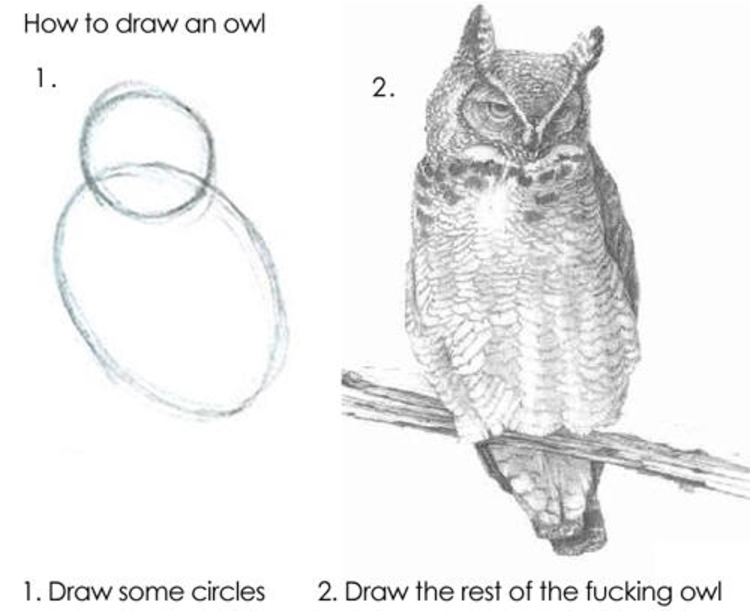
\includegraphics{how-to-draw-an-owl.pdf}
    }
  }
\end{column}%
\end{columns}
\end{frame}

\begin{frame}{Topics to cover}
  \begin{wideitemize}
    \item Spacing and Words
    \item Color
    \item Fonts, Text Size and Readibility
    \item Graphics
    \item Tables
    \item Dummy frames to use as starting points
    \item Misc and options to change
    \item Making an Appendix!
  \end{wideitemize}
\end{frame}



\section{Structure and Spacing}
\begin{transitionframe}
  \begin{center}
    { \Huge \textcolor{black}{Spacing and Words}}
  \end{center}
\end{transitionframe}

\begin{frame}[fragile]{New environments to improve transition and spacing}
\begin{columns}[T] % align columns
\begin{column}{.7\textwidth}

  \begin{wideitemize}
    \item Break up sections using \textcolor{red}{\texttt{transitionframe}} instead of \textcolor{red}{\texttt{frame}}
      { \scriptsize
\begin{verbatim}
\begin{transitionframe}
  \begin{center}
    { \Huge \textcolor{black}{Spacing and Words}}
  \end{center}
\end{transitionframe}
\end{verbatim}
}
    \item  Use my \textcolor{red}{\texttt{wideitemize}} environment instead of \textcolor{red}{\texttt{itemize}}
      \begin{itemize}
      \item This environment automatically spaces wide between items
      \item That way you don't write too much text on a slide!
      \item Rule of thumb 1: \textcolor{green}{45-75 characters a line}
      \item Rule of thumb 2: \textcolor{green}{sentence on one line}
      \end{itemize}
    \item If you use 16:9 perspective, use an image on the side!
  \end{wideitemize}
\end{column}%
\hfill%
\begin{column}{.28\textwidth}
\bigskip
  \makebox[\linewidth][c]{
    \resizebox{\linewidth}{!}{
      
\includegraphics{too-many-words.pdf}
    }
  }
\end{column}%
\end{columns}
\end{frame}

\begin{frame}{Aim for simplicity}
\begin{center}
\Large Better to make one point well on a slide
\end{center}
\end{frame}

\begin{frame}{Than to overwhelm an audience with text}
  \begin{itemize}
  \item \lipsum
  \end{itemize}
\end{frame}

\begin{frame}[fragile]{Roadmap at every section?}
  \begin{wideitemize}
    \item If you prefer to have a roadmap, use the following code:
   \begin{verbatim}[fragile]
 \AtBeginSection[]{%
\begin{frame}%
 \frametitle{Roadmap of Talk}%
 \tableofcontents[currentsection] %
\end{frame}%
}
% \end{verbatim}
    \item This creates a section list at each section marker
    \item I included it in the header -- just uncomment it
  \end{wideitemize}
\end{frame}


\section{Color}
\begin{transitionframe}
  \begin{center}
    { \Huge \textcolor{black}{Color}}
  \end{center}
\end{transitionframe}

\begin{frame}{Colorblindness is an issue}
  \makebox[\linewidth][c]{
    \resizebox{\linewidth}{!}{
      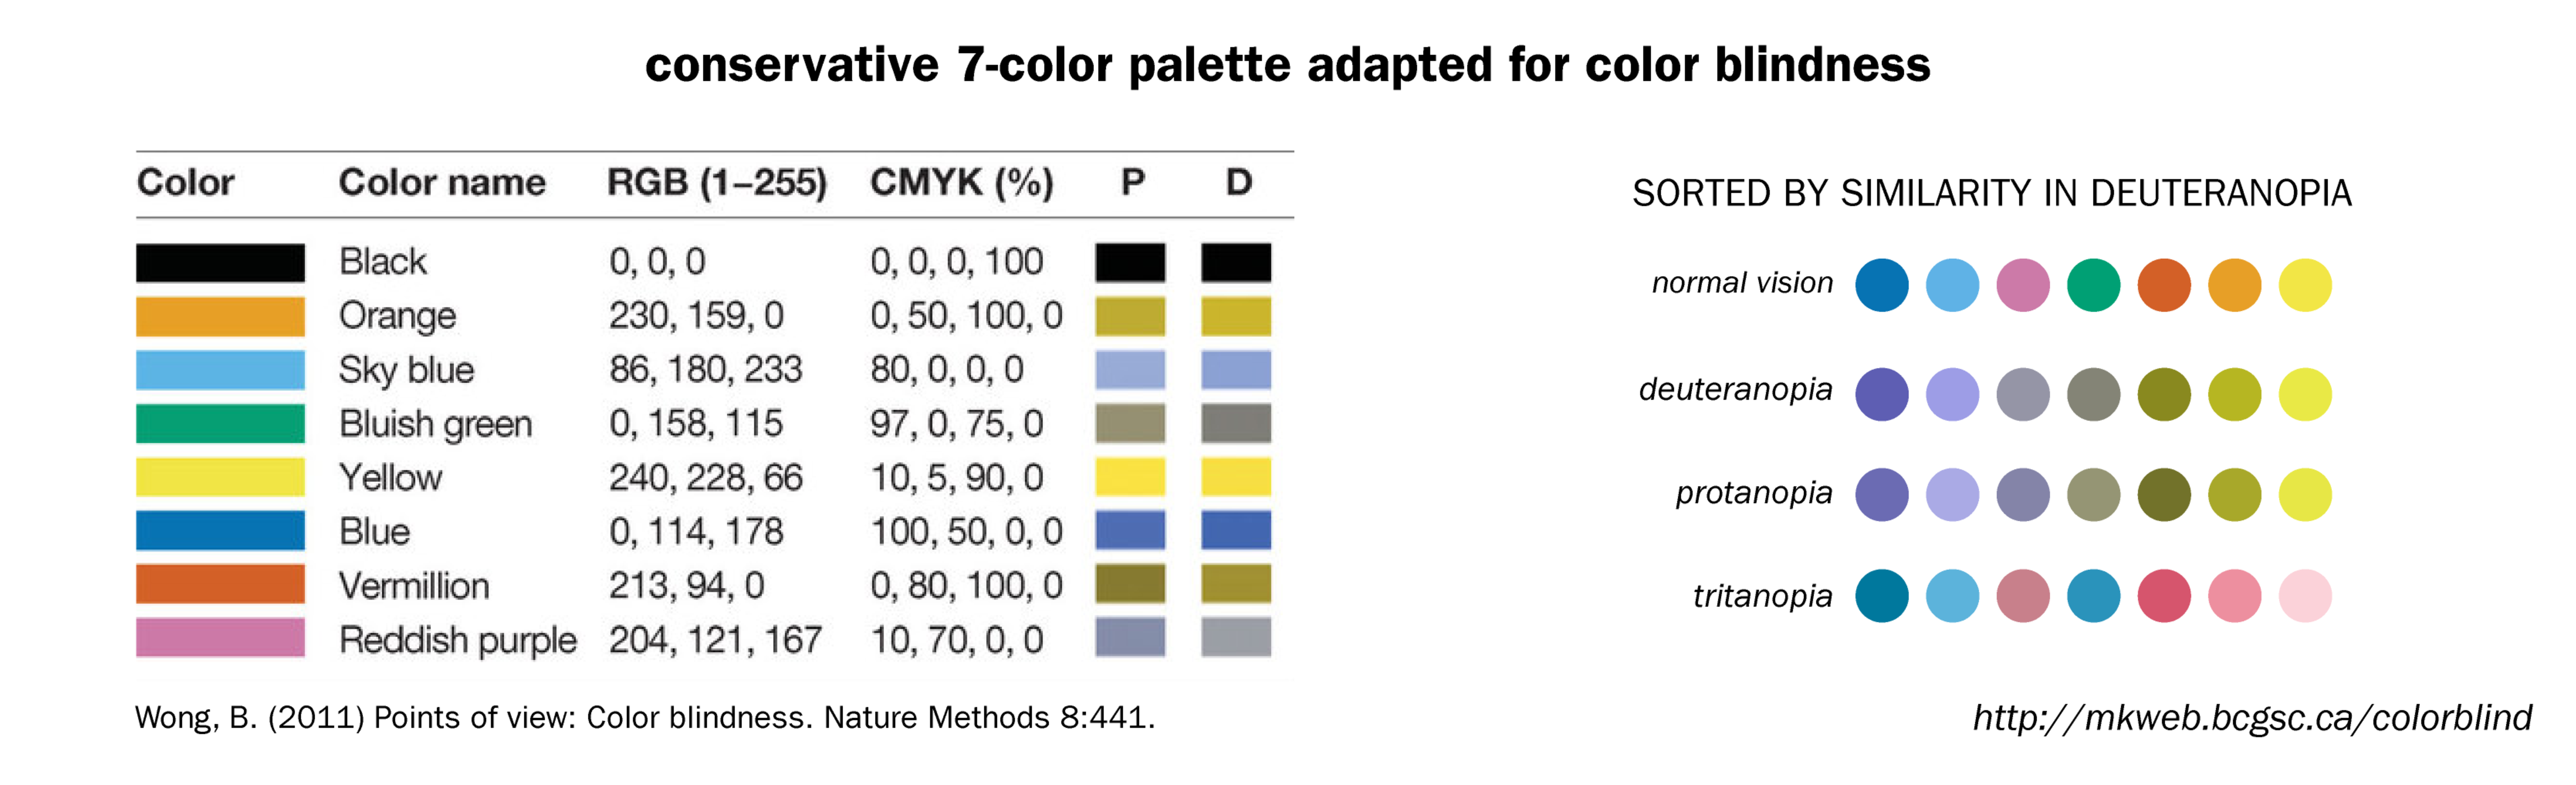
\includegraphics{colorblind.palettes.pdf}
    }
  }
  \begin{itemize}
  \item    The traditional red-blue colors are bad for those who are color blind
  \item    Crib from the above colors!
  \end{itemize}

\end{frame}

\begin{frame}[fragile]{I use two to three colors regularly throughout my presentations}
  \begin{wideitemize}
    \item[-] I use the \textcolor{blue}{blue} color everywhere
    \item[-] I use \textcolor{red}{red}  to contrast and emphasize
    \item[-] I use \textcolor{green}{green}  as a backup
    \item[-] I use \textcolor{yellow}{yellow}  as a transition color
  \end{wideitemize}
\medskip
Make your own color wheel palette!  \url{https://www.sessions.edu/color-calculator/}\\
\end{frame}


\begin{frame}{Background color: I'm undecided}
  \begin{wideitemize}
    \item Changing the background color makes it easier to read
    \item Make your figures in R or Stata have the same background color 
      \begin{itemize}
      \item[] (Or transparent)
      \end{itemize}
    \item In \textcolor{red}{large} auditoriums, go black background with white text
  \end{wideitemize}
\end{frame}

{  \setbeamercolor{background canvas}{bg=black}
\begin{frame}
  \textcolor{white}{Example for an auditorium -- contrast is much higher}
\end{frame}
}
\begin{frame}[fragile]{The color code if you can't find it in the source}
\tiny
\begin{verbatim}
% These are my colors -- there are many like them, but these ones are mine.
\definecolor{blue}{RGB}{0,114,178}
\definecolor{red}{RGB}{213,94,0}
\definecolor{yellow}{RGB}{240,228,66}
\definecolor{green}{RGB}{0,158,115}

%% I use a beige off white for my background
\definecolor{MyBackground}{RGB}{255,253,218}

%% Uncomment this if you want to change the background color to something else
\setbeamercolor{background canvas}{bg=MyBackground}

%% Change the bg color to adjust your transition slide background color!
\newenvironment{transitionframe}{\setbeamercolor{background canvas}{bg=yellow}\begin{frame}}{\end{frame}}


\setbeamercolor{frametitle}{fg=blue}
\setbeamercolor{title}{fg=black}
\setbeamertemplate{footline}[frame number]
\setbeamertemplate{navigation symbols}{} 
\setbeamercolor{itemize item}{fg=blue}
\setbeamercolor{itemize subitem}{fg=blue}
\setbeamercolor{enumerate item}{fg=blue}
\setbeamercolor{enumerate subitem}{fg=blue}
\setbeamercolor{button}{bg=MyBackground,fg=blue}
\end{verbatim}
\end{frame}

\section{Fonts, Text Size and Readibility}
\begin{transitionframe}
  \begin{center}
    \Huge Text Size, Fonts, and Readability
  \end{center}
\end{transitionframe}

\begin{frame}{Text size}
\begin{columns}[T] % align columns
\begin{column}{.58\textwidth}
  \begin{wideitemize}
    \item Don't change the font size to fit the text
    \item You're likely putting too much text if you do
    \item There's really no excuse:
      \begin{itemize}
      \item If you need a busy slide, make it a backup
      \item Then have a link, and click to it
      \item The audience will regret ever doubting you
      \end{itemize}
  \end{wideitemize}
\end{column}
\hfill
\begin{column}{.4\textwidth}
    \resizebox{\linewidth}{!}{
      
\includegraphics{unreadable-slides.pdf}
    }
\end{column}
\end{columns}
\end{frame}

\begin{frame}[label=methodology]{Font size matters for graphs too!}
\begin{columns}[T] % align columns
\begin{column}{.58\textwidth}
\only<1>{
  \makebox[\linewidth][c]{
    \resizebox{\linewidth}{!}{
      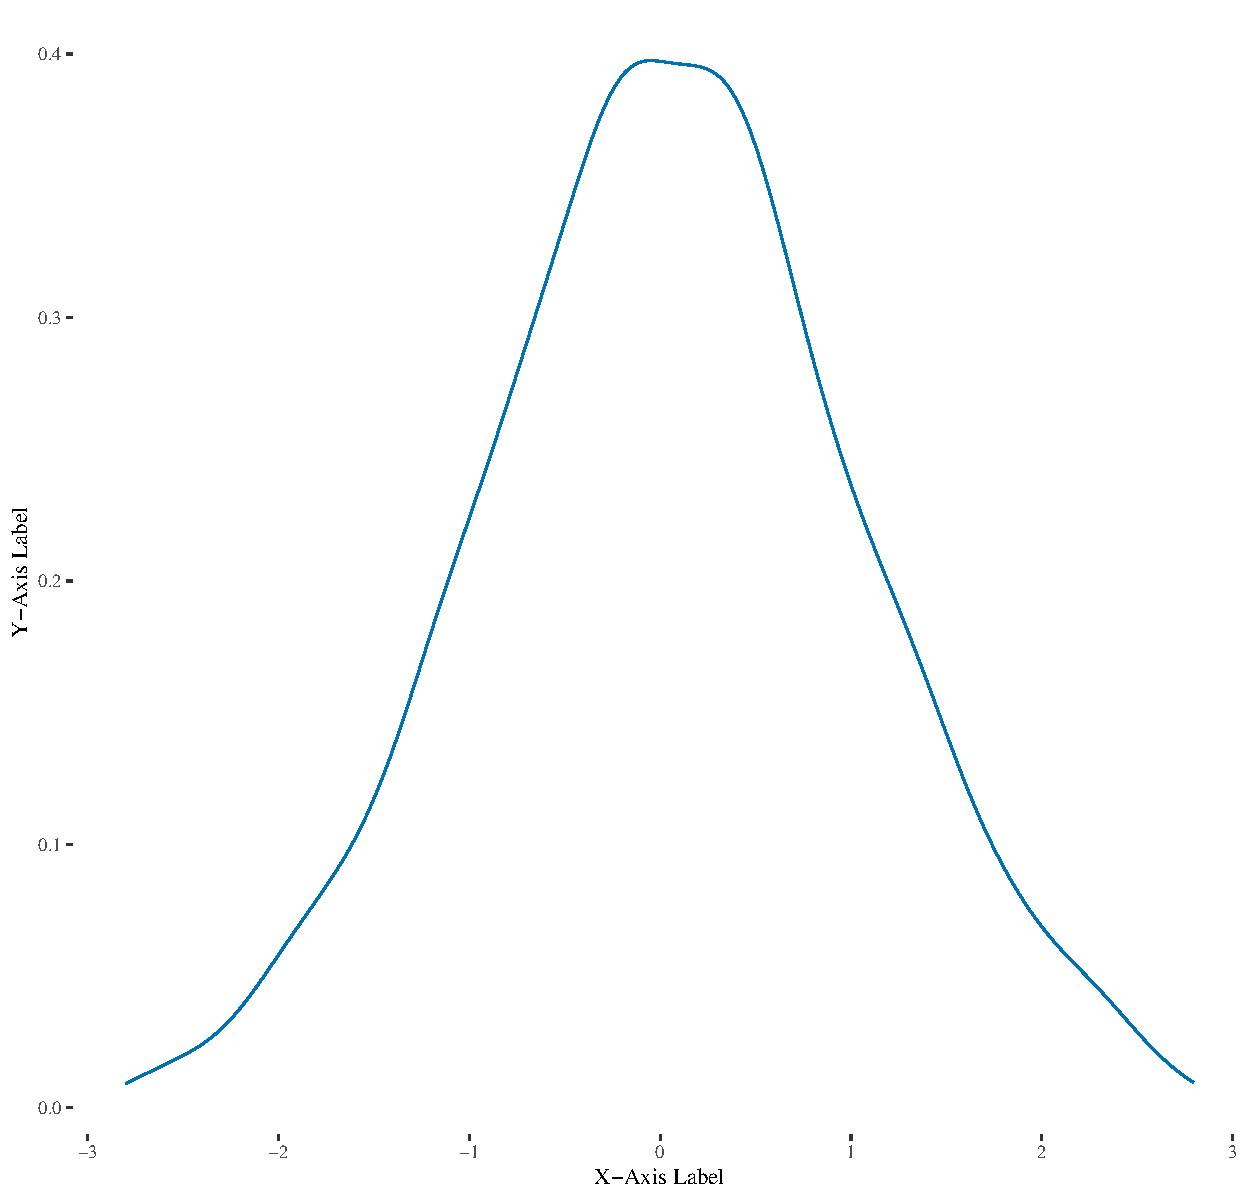
\includegraphics{figure_badlabels.pdf}
    }
  }
}
\only<2>{
  \makebox[\linewidth][c]{
    \resizebox{\linewidth}{!}{
      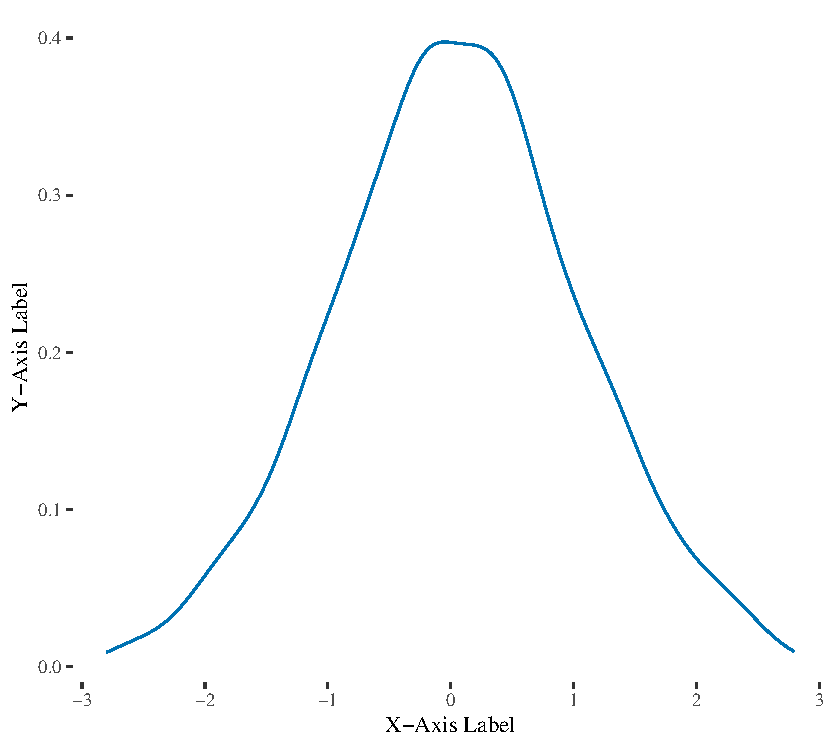
\includegraphics{figure_goodlabels.pdf}
    }
  }
}
\only<3>{
  \makebox[\linewidth][c]{
    \resizebox{\linewidth}{!}{
      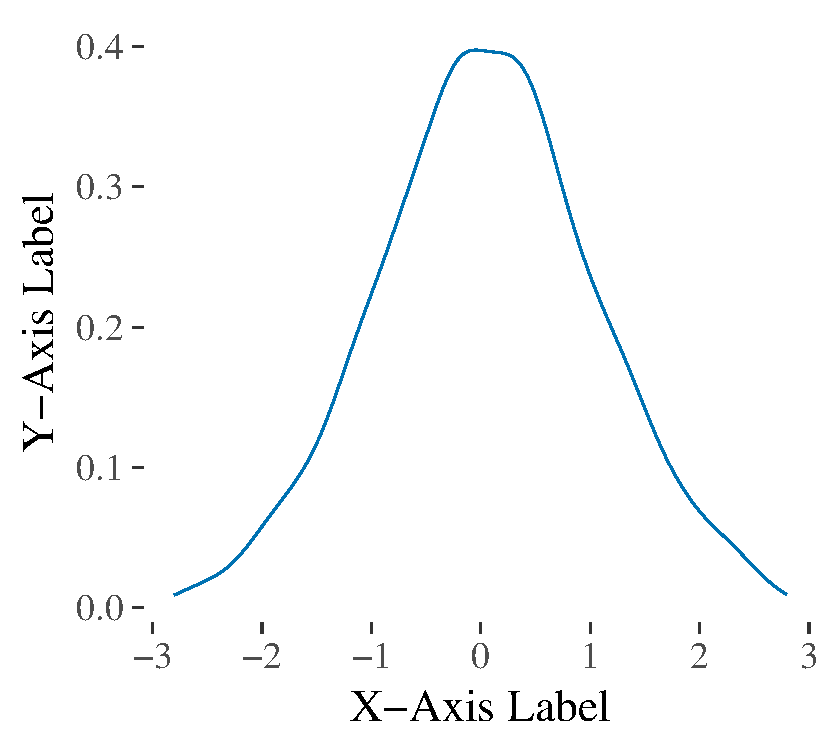
\includegraphics{figure_bestlabels.pdf}
    }
  }
}
\end{column}%
\hfill%
\begin{column}{.4\textwidth}
  \begin{wideitemize}
  \item[]<1-> This graph is unreadable! 
  \item[$\rightarrow$]<1-> Need to change the font size
  \item[]<2-> Now it looks a little better
  \item[]<3-> \textcolor{red}{Much} better 
  \item[]<3-> Things on your computer look too big but audience will thank you
  \end{wideitemize}
\end{column}%
\end{columns}
\end{frame}


\begin{frame}[fragile]{Change your fonts!}
  \begin{wideitemize}
  \item[-] Changing fonts is easy and productive
  \item[-] This slide deck uses Lato -- you can experiment!
  \item[-] Here's some comparison to alternatives:\\
    \begin{itemize}
    \item[]    {Lato: the \textit{quick} \textbf{brown} fox jumps over the $\alpha$- dog}\\
    \item[]     {\fontfamily{cmr}\selectfont  Arial (default): the \textit{quick} \textbf{brown} fox jumps over the $\alpha$- dog}\\
    \item[]     {\fontfamily{pbk}\selectfont  Bookman: the \textit{quick} \textbf{brown} fox jumps over the $\alpha$- dog}\\
    \item[]     {\fontfamily{phv}\selectfont  Helvetica: the \textit{quick} \textbf{brown} fox jumps over the $\alpha$- dog}\\
    \end{itemize}
  \end{wideitemize}
  \bigskip
  To change your font globally, you'll need to find the right package:
  \begin{verbatim}
   \usepackage[default]{lato}
   \end{verbatim}
  Link for choices: \url{http://www.tug.dk/FontCatalogue/sansseriffonts.html}
\end{frame}



\section{Graphics}    
\begin{transitionframe}
  \begin{center}
    \Huge Graphics
  \end{center}
\end{transitionframe}

\begin{frame}[fragile]{Fitting figures doesn't have to be painful}
  \begin{wideitemize}
    \item Simple commands to fit figures: 
    \begin{verbatim}
    \resizebox{0.7\linewidth}{!}{
      \includegraphics{figure1_effect.pdf}}
    \end{verbatim}
    \item The \texttt{\textbackslash linewidth} number is defined within an environment
    \item Simply center with a \texttt{center} environment
  \end{wideitemize}
\end{frame}

\begin{frame}{When possible, make graphic central}
\begin{center}
    \resizebox{0.58\linewidth}{!}{
      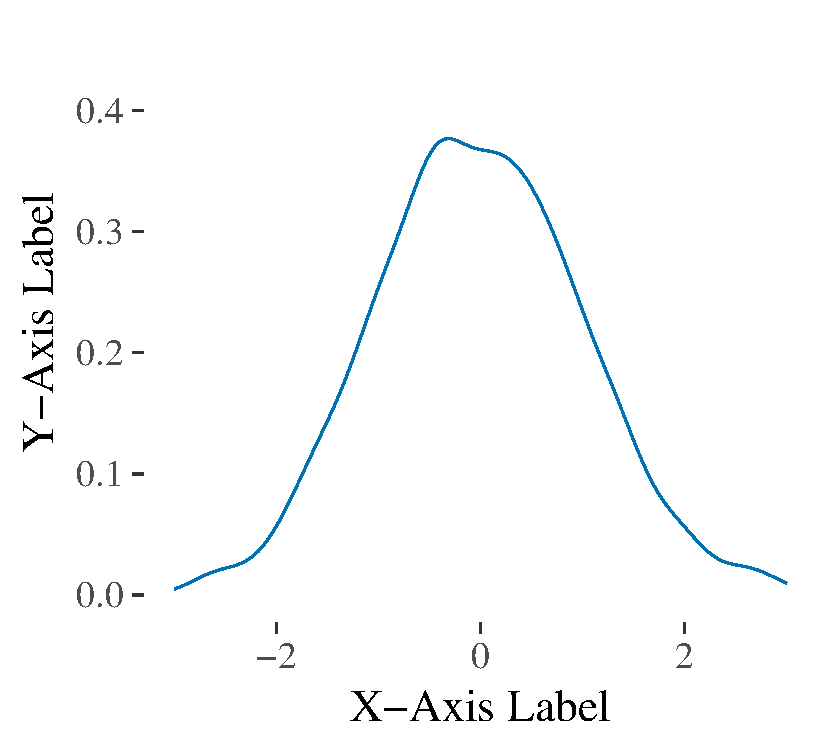
\includegraphics{figure1_overlay.pdf}
    }
\end{center}
\end{frame}
\begin{frame}{But sometimes iteration is better}
\begin{columns}[T]
\begin{column}{.58\textwidth}
    \only<1>{\resizebox{\textwidth}{!}{
      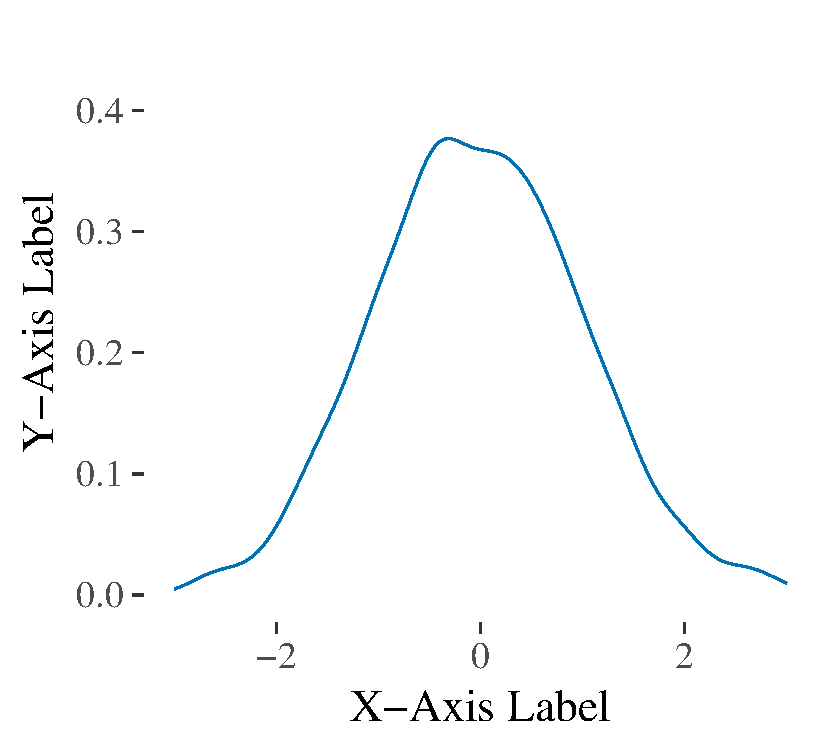
\includegraphics{figure1_overlay.pdf}
    }
  }
    \only<2>{\resizebox{\textwidth}{!}{
      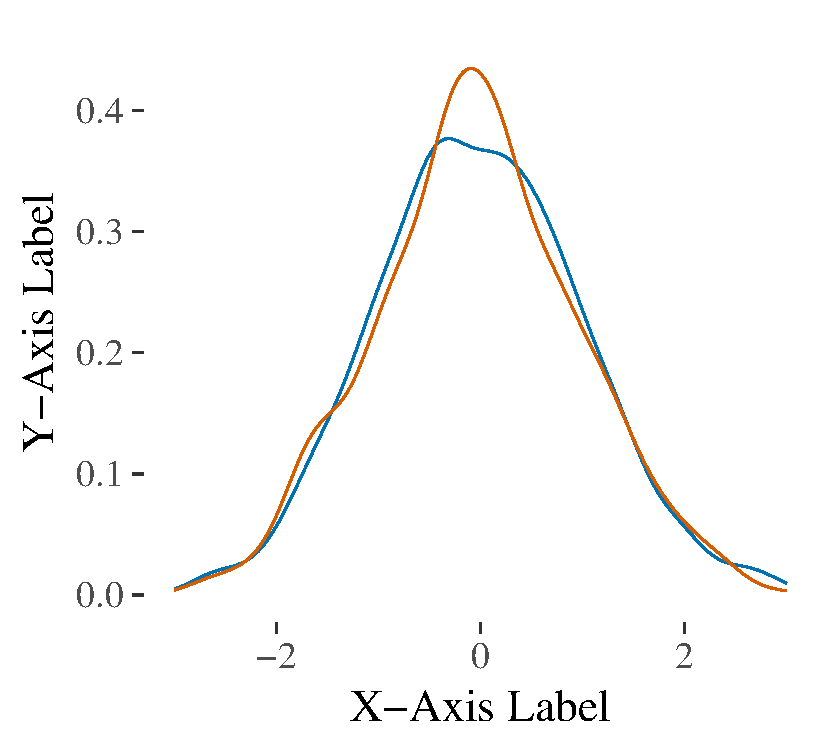
\includegraphics{figure2_overlay.pdf}
    }
  }
    \only<3>{\resizebox{\textwidth}{!}{
      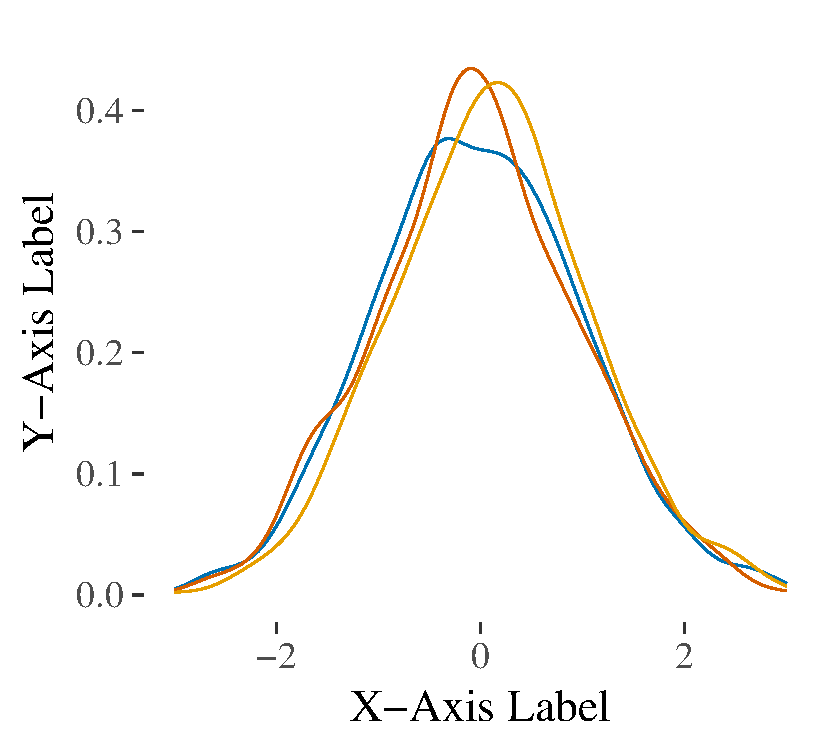
\includegraphics{figure3_overlay.pdf}
    }
  }
\end{column}
\hfill
\begin{column}{.4\textwidth}
  \begin{wideitemize}
  \item<1-> Sometimes you want to talk about one effect
  \item<2-> Then switch to a second effect 
  \item<3-> Use the \texttt{\textbackslash only<slidenum>} command
  \item<3-> For the effect, keep the similar axes
  \end{wideitemize}
  \end{column}
\end{columns}
\end{frame}

\section{Tables}
\begin{transitionframe}
  \begin{center}
    \Huge Tables
  \end{center}
\end{transitionframe}
\begin{frame}[fragile]{Fitting tables doesn't have to be painful}
  \begin{wideitemize}
    \item Simple commands to fit table and center: 
    \begin{verbatim}
\makebox[\linewidth][c]{
\begin{tabular}{l cc ddd}
  results...
\end{tabular}
    \end{verbatim}
    \item Don't use the \texttt{table} environment
    \item If you don't want to center, use change \texttt{[c]} to \texttt{[l]}
  \end{wideitemize}
\end{frame}

\begin{frame}{Highlight cells using tikz (see source code)}
\makebox[\linewidth][c]{
\begin{tabular}{l cc ddd}
  \toprule
  &  Mean at && \multicolumn{3}{c}{Difference-in-Differences Estimates} \\
  \cmidrule{4-6}
  & $ t=-1 $ &&\multicolumn{1}{c}{1 Year} & \multicolumn{1}{c}{2 Years} & \multicolumn{1}{c}{3 Years} \\
  \cmidrule{2-2} \cmidrule{4-6}
  & \multicolumn{1}{c}{(1)}  &&\multicolumn{1}{c}{(2)} & \multicolumn{1}{c}{(3)} & \multicolumn{1}{c}{(4)} \\
  \cmidrule{2-6}
  Outcome 1 & 2.58 && 0.11 &0.08 &\marktopleft{a1} 0.12\\
  & (2.55) && (0.04) & (0.04) & (0.04)\\ 
  Outcome 2 & 60.90 && -0.73 &-1.13 & -1.58\\
  & (17.02) && (0.10) & (0.11) & (0.12)\markbottomright{a1}{red} \\
  Outcome 3 & 18.98 && 0.77 &1.28 & 1.62\\
  & (6.74) && (0.13) & (0.13) & (0.12)\\ 
  \bottomrule
\end{tabular}
}
\uncover<2->{\tikz[overlay,remember picture,inner sep=1pt]
\node[draw=red,rounded corners,fit=(marker-a1-a.north west) (marker-a1-b.south east)] {};}
\end{frame}

\begin{frame}{Reveal rows sequentially using \texttt{\textbackslash onslide} (see source code)}
\makebox[\linewidth][c]{
\begin{tabular}{l cc ddd}
  \toprule
  &  Mean at && \multicolumn{3}{c}{Difference-in-Differences Estimates} \\
  \cmidrule{4-6}
  & $ t=-1 $ &&\multicolumn{1}{c}{1 Year} & \multicolumn{1}{c}{2 Years} & \multicolumn{1}{c}{3 Years} \\
  \cmidrule{2-2} \cmidrule{4-6}
  & \multicolumn{1}{c}{(1)}  &&\multicolumn{1}{c}{(2)} & \multicolumn{1}{c}{(3)} & \multicolumn{1}{c}{(4)} \\
  \cmidrule{2-6}
\onslide<2->{
  Outcome 1 & 2.58 && 0.11 &0.08 & 0.12\\
  & (2.55) && (0.04) & (0.04) & (0.04)
}
\onslide<3->{
\\
  Outcome 2 & 60.90 && -0.73 &-1.13 & -1.58\\
  & (17.02) && (0.10) & (0.11) & (0.12) 
}
\onslide<4>{
\\
  Outcome 3 & 18.98 && 0.77 &1.28 & 1.62\\
  & (6.74) && (0.13) & (0.13) & (0.12)
}
\\\bottomrule
\end{tabular}
}
\begin{itemize}
\item[] There are other ways to do this
\item[] Consider whether it is better to have all the context, or control
\item[] If you haven't practiced, the clicking through slides will be artificial
\end{itemize}

\end{frame}

\begin{frame}{Reveal columns sequentially using \texttt{\textbackslash onslide} (see source code)}
\setbeamercovered{invisible}
\makebox[\linewidth][c]{
\begin{tabular}{l cc <{\onslide<1->}d<{\onslide<2->}d<{\onslide<3->}d<{\onslide}}
  \toprule
  &  Mean at && \multicolumn{3}{c}{Difference-in-Differences Estimates} \\
  \cmidrule{4-6}
  & $ t=-1 $ &&\multicolumn{1}{c}{1 Year} & \multicolumn{1}{c}{2 Years} & \multicolumn{1}{c}{3 Years} \\
  \cmidrule{2-2} \cmidrule{4-6}
  & \multicolumn{1}{c}{(1)}  &&\multicolumn{1}{c}{(2)} & \multicolumn{1}{c}{(3)} & \multicolumn{1}{c}{(4)} \\
  \cmidrule{2-6}
  Outcome 1 & 2.58 && 0.11 &0.08 & 0.12\\
  & (2.55) && (0.04) & (0.04) & (0.04)\\ 
  Outcome 2 & 60.90 && -0.73 &-1.13 & -1.58\\
  & (17.02) && (0.10) & (0.11) & (0.12) \\
  Outcome 3 & 18.98 && 0.77 &1.28 & 1.62\\
  & (6.74) && (0.13) & (0.13) & (0.12)\\
\bottomrule
\end{tabular}
}

\begin{itemize}
\item[] This is a bit more difficult to get working every time, but can be very nice
\item[] Just don't overuse it
\item[] You can even talk about your results down here!
\end{itemize}
\end{frame}


\section{Dummy Frames}
\begin{transitionframe}
  \begin{center}
    \Huge Dummy Frames
  \end{center}
\end{transitionframe}


\begin{frame}{Here's a list of frames that are similar to powerpoint frames}
  \begin{wideitemize}
    \item Just copy and paste the source code
  \end{wideitemize}
\end{frame}


\begin{frame}{Two Column Frame}
\begin{columns}[T] % align columns
\begin{column}{.58\textwidth}
\color{red}\rule{\linewidth}{4pt}
Column 1
\end{column}%
\hfill%
\begin{column}{.38\textwidth}
\color{blue}\rule{\linewidth}{4pt}
Column 2
\end{column}%
\end{columns}
\end{frame}

\begin{frame}
  \vspace{-8pt}
\begin{columns}[T] % align columns
\begin{column}{.58\textwidth}
\begin{minipage}[t][\textheight][t]
  {\dimexpr\textwidth}
  \vspace{8pt}
  \hspace{4pt} \textcolor{blue}{Two Column w/ Face}
  \vspace{8pt}
  
Information goes here
    \end{minipage}
\end{column}%
\hfill%
\begin{column}{.42\textwidth}
 \colorbox{green!20}{\begin{minipage}[t][1.2\textheight][t]
      {\dimexpr\textwidth}
      Face goes here
    \end{minipage}}
\end{column}%
\end{columns}
\end{frame}

\begin{videoframe}{This Looks Good}
  Using the Environ package
\end{videoframe}

\begin{frame}{Table Frame}
\setbeamercovered{invisible}
\makebox[\linewidth][c]{
\begin{tabular}{l}
\toprule
Temp Table\\
\bottomrule
\end{tabular}
}
\end{frame}

\begin{frame}{Figure Frame}
\begin{center}
\resizebox{0.5\textwidth}{!}{
  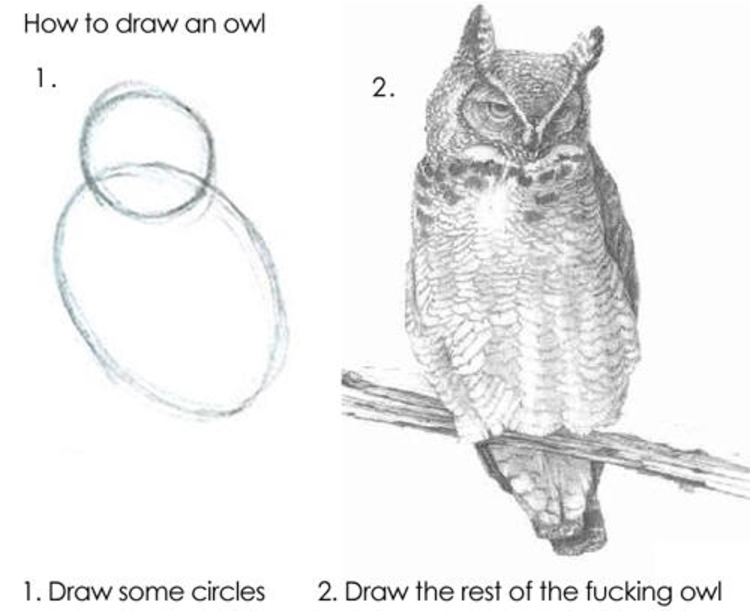
\includegraphics{how-to-draw-an-owl.pdf}
}
\end{center}
\end{frame}

\begin{frame}{Figure with Commentary Frame}
\begin{columns}[T] % align columns
\begin{column}{.58\textwidth}
\resizebox{\textwidth}{!}{
  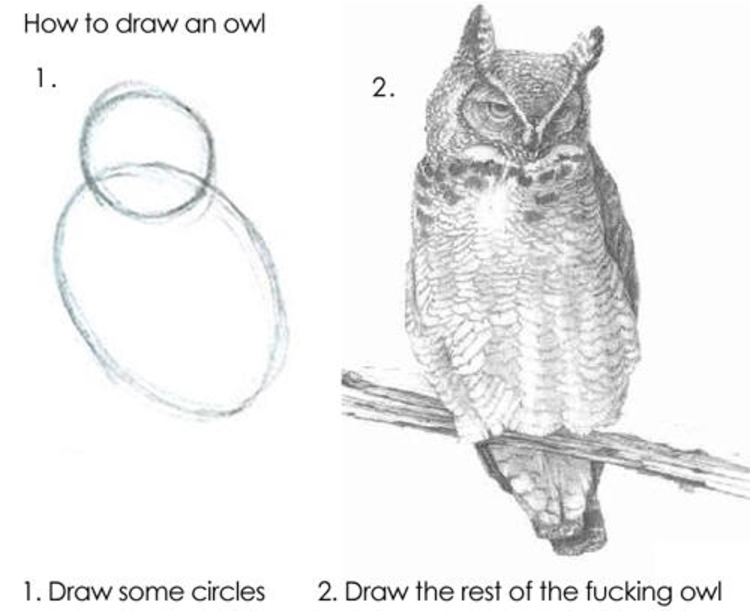
\includegraphics{how-to-draw-an-owl.pdf}
}
\end{column}%
\hfill%
\begin{column}{.38\textwidth}
  \begin{wideitemize}
  \item Everyone gives these tips on nice presentations
  \item But maybe we'd put less on the slides
  \item If the audience stopped interrupting
  \end{wideitemize}
\end{column}%
\end{columns}
\end{frame}


\section{Misc and options to change}
\begin{transitionframe}
  \begin{center}
    \Huge Miscellaneous + Options
  \end{center}
\end{transitionframe}

\begin{frame}{Make TikZ figures to help highlight your research design}
  \begin{wideitemize}
    \item Previously used tikz commands to highlight things in figures and tables
    \item You can make much cooler figures with this
    \item Here's an example for showing diff-in-diff timing:
  \end{wideitemize}
\begin{center}
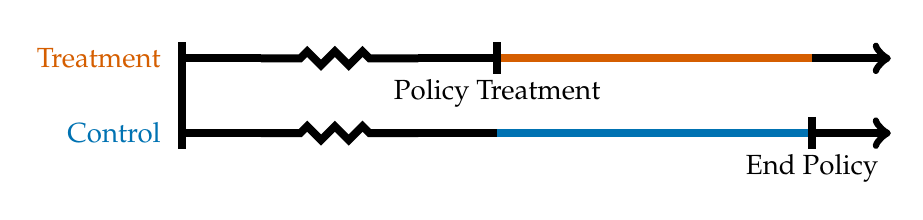
\begin{tikzpicture}[snake=zigzag, line before snake = 5mm, line after snake = 5mm, line width=1mm]
    % draw horizontal line   
    \draw (0,0) -- (1,0);
    \draw[snake] (1,0) -- (3,0);
    \draw (3,0) -- (4,0);
    \draw[blue] (4,0) -- (8,0);
    \draw[->] (8,0) -- (9,0);


    \draw (0,.95) -- (1,.95);
    \draw[snake] (1,.95) -- (3,.95);
    \draw (3,.95) -- (4,.95);
    \draw[red] (4,.95) -- (8,.95);
    \draw[->] (8,.95) -- (9,.95);

    % draw vertical lines
    \foreach \x in {8}
      \draw (\x cm,.205) -- (\x cm,-.205);
    \foreach \x in {4}
      \draw (\x cm,{.95+(.205)}) -- (\x cm,{.95-(.205)});
    \foreach \x in {0}
      \draw (\x cm,{.95+(.205)}) -- (\x cm,{0-(.205)});

    % draw nodes
    \draw (0,0) node[below=.105] {}  node[left=.105] {\textcolor{blue}{Control}};
    \draw (0,0.95) node[below=.105] {} node[above=.105] {} node[left=.105] {\textcolor{red}{Treatment}};
    \draw (4,.95) node[below=.105] {} node[above=.105] {} node[below=.105] {Policy Treatment};
    \draw (8,0) node[below=.105] {} node[above=.105] {} node[below=.105] {End Policy};
  \end{tikzpicture}
\end{center}
\end{frame}

\begin{frame}{Consider making your math prettier}
  \begin{wideitemize}
    \item Don't overdo it when putting up equations\\(either regressions or theorems)
    \item Try adding color and text to highlight the relevant formula
    \item Consider (Imbens and Angrist 1994): 
      \begin{equation*}
        \alpha_{g}^{IV} = \left. \underbrace{Cov(Y, g(\textcolor{blue}{Z}))}_{\text{\textcolor{red}{Reduced Form}}} \middle/ \underbrace{Cov(D, g(\textcolor{blue}{Z}))}_{\text{\textcolor{green}{First Stage}}} \right.
      \end{equation*}
  \end{wideitemize}
\end{frame}


\begin{frame}{Notes for yourself}
  \begin{wideitemize}
    \item An underused feature of beamer is the notes feature
    \item Outside of frame environment, you use the \texttt{\textbackslash note} command
    \item See the source code after this frame, and in the header
    \item You can even make these notes available for you as you present!
  \end{wideitemize}
\begin{center}
  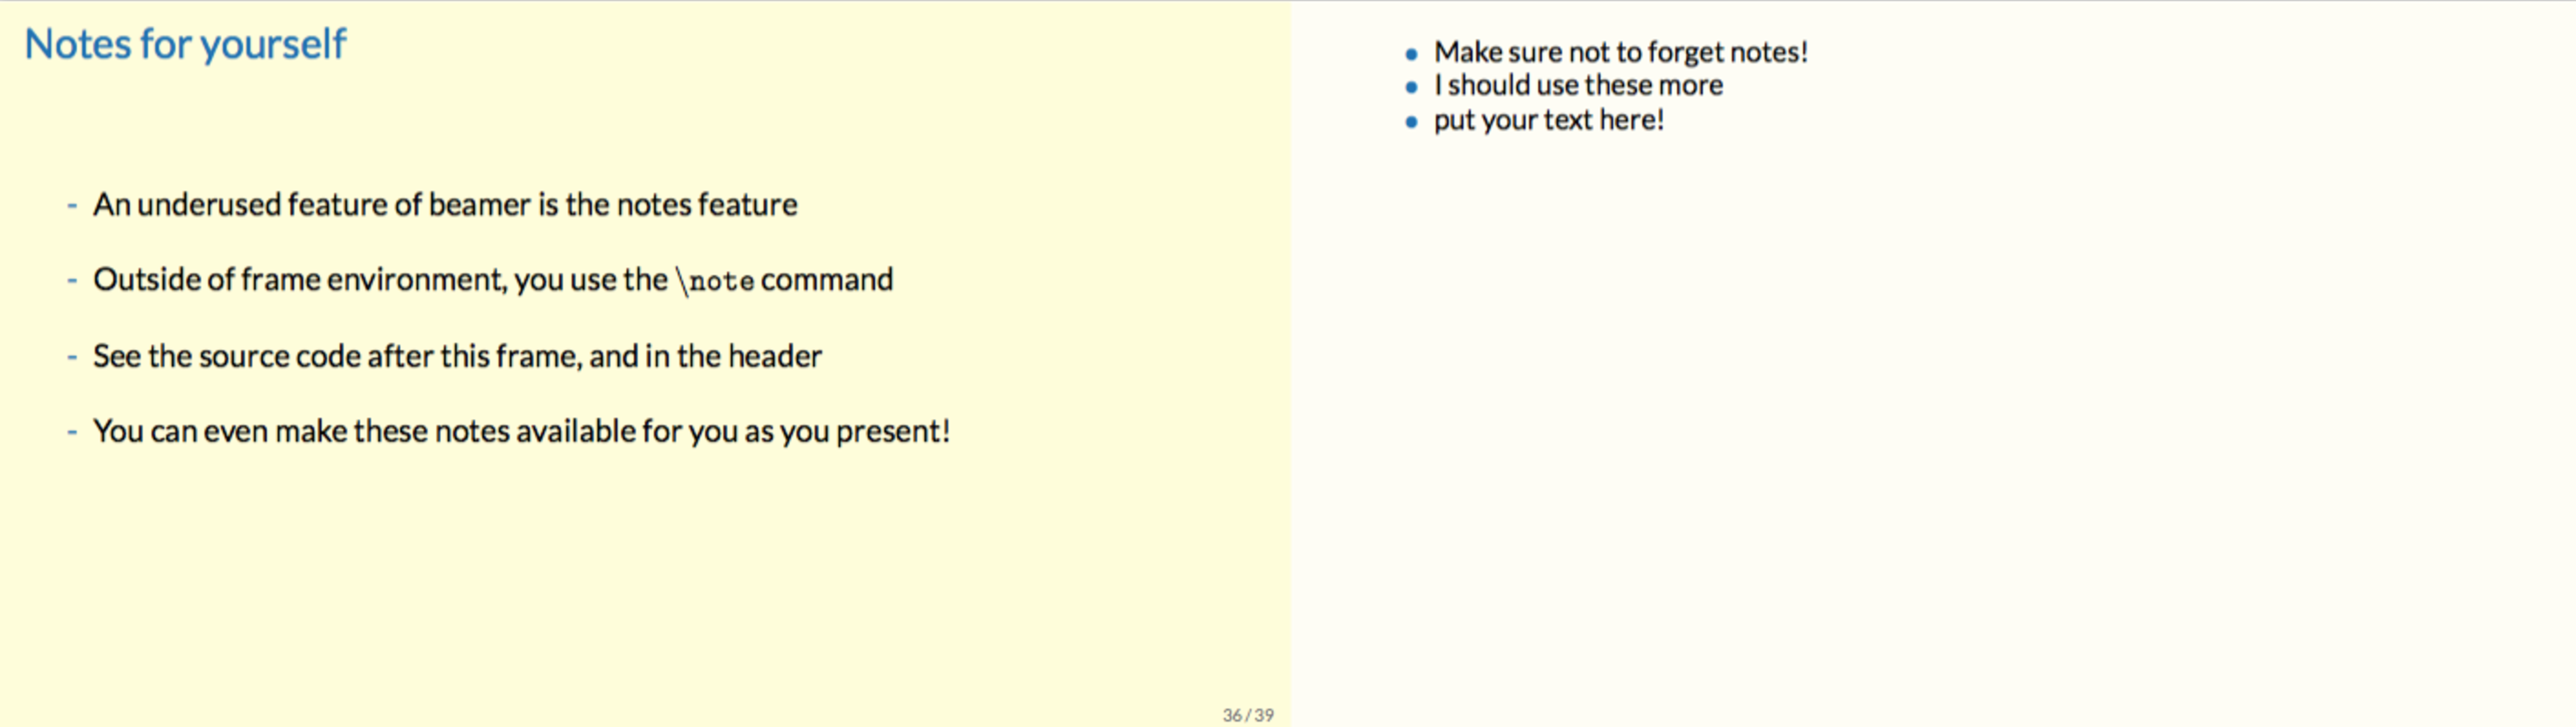
\includegraphics[width=.9\linewidth]{example_note.pdf}
\end{center}
\end{frame}
% From here: https://tex.stackexchange.com/questions/114219/add-notes-to-latex-beamer
% To give a presentation with the Skim reader (http://skim-app.sourceforge.net) on OSX so
% that you see the notes on your laptop and the slides on the projector, do the following:
% 
% 1. Generate just the presentation (hide notes) and save to slides.pdf
% 2. Generate onlt the notes (show only nodes) and save to notes.pdf
% 3. With Skim open both slides.pdf and notes.pdf
% 4. Click on slides.pdf to bring it to front.
% 5. In Skim, under "View -> Presentation Option -> Synhcronized Noted Document"
%    select notes.pdf.
% 6. Now as you move around in slides.pdf the notes.pdf file will follow you.
% 7. Arrange windows so that notes.pdf is in full screen mode on your laptop
%    and slides.pdf is in presentation mode on the projector.
\note[itemize]{
\item Make sure not to forget notes!
\item I should use these more
\item put your text here!
}


\begin{frame}{Sizing / perspective on frame}
  \begin{wideitemize}
  \item Thanks to Casey Wichman, these slides are in beautiful 16:9
  \item If you don't want that, just remove the \texttt{aspectratio} option in the document class
  \item But, it will be hard to put stuff next to pictures
  \item It's much more modern looking in 16:9
  \end{wideitemize}
\end{frame}

\section{Appendix}
\begin{transitionframe}
  \begin{center}
    \Huge Appendix!
  \end{center}
\end{transitionframe}

\begin{frame}{Almost done!}
  \begin{wideitemize}
  \item Use the \texttt{\textbackslash appendix} command to restart the numbering
  \item The frame counter says this is the last slide, but it's not
  \item (Test it, see you on next page)
  \end{wideitemize}
\end{frame}

\appendix

\begin{frame}[label=appendix_start]{Almost done!}
  \begin{wideitemize}
  \item See, now we're in backup slide land
  \item This is made useful by having links throughtout the talk
  \item Here's a button, which is how I make links \hyperlink{appendix_end}{\beamergotobutton{Next slide}}
  \end{wideitemize}
\end{frame}

\begin{frame}[label=appendix_end]{Use it to intimidate audiences!}
  \begin{wideitemize}
    \item[] Now you can make it clear you've done a shitload of work
      \begin{itemize}
      \item[]  without having to show everything! \hyperlink{appendix_start}{\beamergotobutton{Back}}
      \end{itemize}
    \item[] You label a frame with the \texttt{[label=name]} option, and then point a link to it
    \item[] You can make an object a link using the \texttt{\textbackslash hyperlink\{label\}\{object\}} command
  \end{wideitemize}
\end{frame}



\end{document}
